
\documentclass[a4paper]{article}

% F O N T S
\usepackage[T1]{fontenc}  % Use T1 encoded cm-super fonts.
\usepackage{microtype}    % Improve typesetting.
\usepackage{fix-cm}       % Support for arbitrary font size for cm.
\usepackage{xspace}
\usepackage{listings}
\lstset{numbers=left,basicstyle=\small,language=Tex}

% P A G E   L A Y O U T
% Use geometry package to set up margins.
% A4 paper is 8.27 × 11.69 inch.
\RequirePackage[a4paper, width=6.27in, height=9.69in, includehead]{geometry}

% Set line spacing.
\RequirePackage{setspace}
\onehalfspacing

% Setup the hyperref package for enabling links, bookmarks, and PDF properties.
\RequirePackage[hyphens]{url} % Embedding URL's in document.
\RequirePackage[bookmarks=true]{hyperref}
\hypersetup
{
	pdfstartview = {FitV},
	pdfpagemode  = UseNone,
	colorlinks   = true,
	linkcolor    = red,
	citecolor    = blue,
	filecolor    = magenta,
	urlcolor     = cyan
}

% C L E V E R E F
% 
% Must come as late as possible, especially after hyperref.
\RequirePackage[capitalize]{cleveref}

% Disable the automatic abbreviations of equations and figures.
\crefname{equation}{Equation}{Equations}
\crefname{figure}{Figure}{Figures}
\Crefname{equation}{Equation}{Equations}
\Crefname{figure}{Figure}{Figures}

% Change the way links are produced in PDF documents.
\crefformat{chapter}{#2Chapter~#1#3}
\crefformat{section}{#2Section~#1#3}
\crefformat{figure}{#2Figure~#1#3}
\crefformat{equation}{#2Equation~#1#3}
\crefformat{table}{#2Table~#1#3}
\Crefformat{chapter}{#2Chapter~#1#3}
\Crefformat{section}{#2Section~#1#3}
\Crefformat{figure}{#2Figure~#1#3}
\Crefformat{equation}{#2Equation~#1#3}
\Crefformat{table}{#2Table~#1#3}
\creflabelformat{equation}{#2#1#3}

% Set the front page matter.

\newcommand{\SgTitle}[1]{\hypersetup{pdftitle={#1}}\title{#1}}
\newcommand{\SgAuthor}[1]{\hypersetup{pdfauthor={#1}}}
\newcommand{\SgSubject}[1]{\hypersetup{pdfsubject={#1}}}
\newcommand{\SgKeywords}[1]{\hypersetup{pdfkeywords={#1}}}

\newcommand{\SgFrontMatter}[3]%
{%
	\SgTitle{#1}%
	\SgAuthor{#2}%
	\author{#2 (#3)}
	\maketitle%
	\tableofcontents%
}

\newcommand{\SPhdThesis}{\textbf{SPhdThesis}\xspace}
\newcommand{\Code}[1]{\texttt{#1}\xspace}

\begin{document}
\SgFrontMatter{SPhdThesis class documentation}{Saurabh Garg}{\url{saurabhgarg@mysoc.net}}
\SgKeywords{PhD thesis; latex template; SoC; NUS}

\section{Introduction}
I developed \SPhdThesis document class while writing my PhD thesis in School of Computing (SoC), National University of Singapore (NUS). By default, it adheres to the ``NUS Guidelines on Format of Research Thesis Submitted For Examination'' located at \url{http://www.nus.edu.sg/registrar/event/gd-thesisexam.html}\footnote{You need NUSNET username and password to access the document.}. However, it is quite easy to change it for different guidelines. Section~\ref{sec:GettingStarted} (Getting started) describes how to quickly start using \SPhdThesis with default options. The class options used to customize the formatting of the thesis are described in Section~\ref{sec:ClassOptions}. Section~\ref{sec:Tweaking} gives some hints for tweaking the class file and Section~\ref{sec:Issues} list the currently know issues. Although, not related to this document class, Section~\ref{sec:Tools} lists some tools I find useful for working with \LaTeX. \\

An important point to consider before using this document class is that it only supports using \texttt{pdflatex}. It cannot be used with \texttt{latex} to create a dvi file. The implication of using pdflatex is that all your figures have to be in pdf, png or jpg. You cannot use eps figures. However, there are tools to convert eps files to pdf on all platforms.

\section{Getting started}\label{sec:GettingStarted}
The easiest way to start using \SPhdThesis document class is to copy \texttt{SPhdThesis.cls} and \texttt{example\textbackslash{}} \texttt{thesis.tex} to your thesis folder and modify \texttt{thesis.tex}. The following is the complete listing of \texttt{thesis.tex}:

\begin{lstlisting}
\documentclass{SPhdThesis}

% Title page and PDF properties.
\SgSetTitle{A Robust Mesh-based Surface Integration Algorithm}
\SgSetAuthor{Saurabh Garg}
\SgSetAuthorDegrees{List your previous degrees here}
\SgSetYear{2013}
\SgSetDegree{Doctor of Philosophy}
\SgSetDepartment{Department of Computer Science}
\SgSetUniversity{National University of Singapore}
\SgSetDeclarationDate{June 2013}

% The document.
\begin{document}
	\begin{frontmatter}
		\SgAddTitle%
		\SgAddDeclaration%
		%%% Acknowledgements
%%% ----------------------------------------------------------------------
\begingroup
% you can erase the following three lines if you do not use an introductory quote
\cleardoublepage
\let\clearpage\relax
\let\cleardoublepage\relax
\begin{flushright}\slshape
	Put your fancy quote here. Or don't. \\ \medskip
	--- Awesome Author
\end{flushright}

\bigskip
\otherlanguage{ngerman}

\addchap{Vorwort}

\blindmathfalse
\blindtext

\bigskip

\begin{flushright}
	Place, \doctime
\end{flushright}

\endgroup%
		% !TEX root = main.tex
% !TEX encoding = Windows Latin 1
% !TEX TS-program = pdflatex
% 
% Archivo: abstract.tex (en ingles)


\chapter{Abstract} % No cambiar el titulo
\selectlanguage{english}
\noindent
Duis tristique sollicitudin leo nec consequat. Praesent et dui convallis velit tincidunt fermentum. Mauris cursus purus at sem viverra sed imperdiet sapien imperdiet. Aliquam mattis, elit eget rutrum vulputate, tortor sem pulvinar justo, sit amet mollis felis sem at nibh. Donec malesuada, neque id interdum eleifend, arcu augue porta elit, nec tristique libero metus at massa. Fusce fringilla laoreet rhoncus. Suspendisse potenti. Phasellus dignissim sodales mauris at pharetra. Donec gravida fringilla velit ac rutrum.

Curabitur ornare lectus id diam molestie eu imperdiet nulla tempus. Maecenas vestibulum enim et dui ornare blandit. Vivamus fermentum faucibus viverra. Maecenas at justo sapien. Aenean rhoncus augue mattis purus rhoncus venenatis. Suspendisse metus felis, porttitor in varius in, vulputate at tortor. Aliquam molestie, turpis et malesuada porta, tortor sapien pharetra sapien, ac rhoncus quam dolor a sapien. Pellentesque varius laoreet enim ut auctor. Nullam nec ultricies nisi. Nullam porta lectus et ante consectetur posuere.

Duis tristique sollicitudin leo nec consequat. Praesent et dui convallis velit tincidunt fermentum. Mauris cursus purus at sem viverra sed imperdiet sapien imperdiet. Aliquam mattis, elit eget rutrum vulputate, tortor sem pulvinar justo, sit amet mollis felis sem at nibh. Donec malesuada, neque id interdum eleifend, arcu augue porta elit, nec tristique libero metus at massa. Fusce fringilla laoreet rhoncus. Suspendisse potenti. Phasellus dignissim sodales mauris at pharetra. Donec gravida fringilla velit ac rutrum.

Duis tristique sollicitudin leo nec consequat. Praesent et dui convallis velit tincidunt fermentum. Mauris cursus purus at sem viverra sed imperdiet sapien imperdiet. Aliquam mattis, elit eget rutrum vulputate, tortor sem pulvinar justo, sit amet mollis felis sem at nibh. Donec malesuada, neque id interdum eleifend, arcu augue porta elit, nec tristique libero metus at massa. Fusce fringilla laoreet rhoncus. Suspendisse potenti. Phasellus dignissim sodales mauris at pharetra. Donec gravida fringilla velit ac rutrum.

Curabitur ornare lectus id diam molestie eu imperdiet nulla tempus. Maecenas vestibulum enim et dui ornare blandit. Vivamus fermentum faucibus viverra. Maecenas at justo sapien. Aenean rhoncus augue mattis purus rhoncus venenatis. Suspendisse metus felis, porttitor in varius in, vulputate at tortor. Aliquam molestie, turpis et malesuada porta, tortor sapien pharetra sapien, ac rhoncus quam dolor a sapien. Pellentesque varius laoreet enim ut auctor. Nullam nec ultricies nisi. Nullam porta lectus et ante consectetur posuere.

Duis tristique sollicitudin leo nec consequat. Praesent et dui convallis velit tincidunt fermentum. Mauris cursus purus at sem viverra sed imperdiet sapien imperdiet. Aliquam mattis, elit eget rutrum vulputate, tortor sem pulvinar justo, sit amet mollis felis sem at nibh. Donec malesuada, neque id interdum eleifend, arcu augue porta elit, nec tristique libero metus at massa. Fusce fringilla laoreet rhoncus. Suspendisse potenti. Phasellus dignissim sodales mauris at pharetra. Donec gravida fringilla velit ac rutrum.

\bigskip
\noindent
\textit{Key words:} first word; second word; third word.
% Separar palabras con punto-y-comas.

\checklanguage
% Fin archivo abstract.tex
\endinput %
		\SgAddToc% Add table of contents.
		\SgAddLof% Add list of figures.
		\SgAddLot% Add list of tables.
		\SgAddLoa% Add list of algorithms.
	\end{frontmatter}
   
	%
% Modified by Sameer Vijay
% Last Change: Tue Jul 26 2005 13:00 CEST
%
%%%%%%%%%%%%%%%%%%%%%%%%%%%%%%%%%%%%%%%%%%%%%%%%%%%%%%%%%%%%%%%%%%%%%%%%
%
% Sample Notre Dame Thesis/Dissertation
% Using Donald Peterson's ndthesis classfile
%
% Written by Jeff Squyres and Don Peterson
%
% Provided by the Information Technology Committee of
%   the Graduate Student Union
%   http://www.gsu.nd.edu/
%
% Nothing in this document is serious except the format.  :-)
%
% If you have any suggestions, comments, questions, please send e-mail
% to: ndthesis@gsu.nd.edu
%
%%%%%%%%%%%%%%%%%%%%%%%%%%%%%%%%%%%%%%%%%%%%%%%%%%%%%%%%%%%%%%%%%%%%%%%%


%
% Chapter 1
%

\chapter{INTRODUCTION}

\section{Overview}

This is an overview of the introduction.  In here, I will use many
many buzzwords and other legalistic-types of terms, mostly begining on
the expounding of the holistic and synergistic energy that Gnus bring
to our organizations.

\subsection{Background}

In preparation for reading this dissertation, I would highly recommend
reading some of the other material available on
Gnus~\citep{gnus98:_gerry_ganst,greenfield96:_gettin_know_gnu}.  They
are very well written and will give you a fuller understanding of
Gnus.

Gnus are frequently mistakes for squirrels.  They are not squirrels.
They are Gnus.  Don't call them squirrels, either (unless you have
food in your hand); they tend to get a bit upset.\footnote{This is
  frequently mistaken for the chattering and scampering away.  Gnus
  are actually quite polite; they will leave if they have nothing nice
  to say, for fear of saying something offensive.}  If you have food
in your hand, they tend to ignore this insult and accept your food as
a peace offering.

\subsection{Foreground}

Table~\ref{tbl:bogus1} shows some feeding frequencies for where Gnus
like to eat around the Notre Dame campus.  Gnus have work weeks, just
like humans do, hence the much lower frequencies on weekends.  This
can lead us to conclude that Gnu weekend shifts are much smaller than
the normal work-week shifts.  In fact, we can attempt to parametrize the
sighting frequency, $\mathcal{F}$, by the student population, type of food, and
day of the week as:
\begin{equation}
  \mathcal{F} = \mathcal{F}(p,f,d).
\end{equation}
Table~\ref{tbl:bogus2} shows what they
typically like to eat.

\begin{table}[tpb]
  \begin{center}
    \caption{WHERE Gnus LIKE TO EAT \label{tbl:bogus1}}
    \begin{tabularx}{0.85\textwidth}{lrrrrrrr} \toprule
      \multicolumn{1}{c}{Location} & Sun & Mon & Tue & Wed & Thu & Fri & Sat \\ \midrule
      Front of Dome & 1 & 5 & 6 & 5 & 4 & 5 & 1 \\
      Stonehenge & 2 & 9 & 10 & 12 & 9 & 14 & 2 \\
      The Rock & 1 & 3 & 4 & 3 & 4 & 3 & 0 \\
      The ACC & 3 & 4 & 5 & 5 & 5 & 4 & 1 \\
      Dining Halls & 5 & 14 & 12 & 13 & 14 & 12 & 3 \\
      Hesburgh Library & 2 & 3 & 5 & 2 & 3 & 4 & 2 \\ \bottomrule
    \end{tabularx}
  \end{center}
\end{table}

\begin{table}[tpb]
  \setlength{\capwidth}{0.7\textwidth}
  \begin{center}
    \caption{WHAT Gnus LIKE TO EAT ON THE NOTRE DAME CAMPUS, LISTED
      BY AVERAGE NUMBER OF SIGHTINGS PER WEEKDAY
    \label{tbl:bogus2}
}
    \begin{tabular}{lrrrrrrr} \toprule
      \multicolumn{1}{c}{Food} & Sun & Mon & Tue & Wed & Thu & Fri & Sat \\ \midrule
      Twinkies & 1 & 5 & 6 & 5 & 4 & 5 & 1 \\
      Ding Dongs & 2 & 9 & 10 & 12 & 9 & 14 & 2 \\
      Carrots & 1 & 3 & 4 & 3 & 4 & 3 & 0 \\
      Lettuce & 3 & 4 & 5 & 5 & 5 & 4 & 1 \\
      Twizlers & 5 & 14 & 12 & 13 & 14 & 12 & 3 \\
      Jawbreakers & 2 & 3 & 5 & 2 & 3 & 4 & 2 \\ \bottomrule
    \end{tabular}
  \end{center}
\end{table}

Figure~\ref{fig:bogus3} shows a nice graph of location distributions
by day of week.  I have no real reason for including it except to show
that figures work as well.  Did I mention that Gnus are really cool?

\begin{figure}[tpb]
  \begin{center}
    \centerline{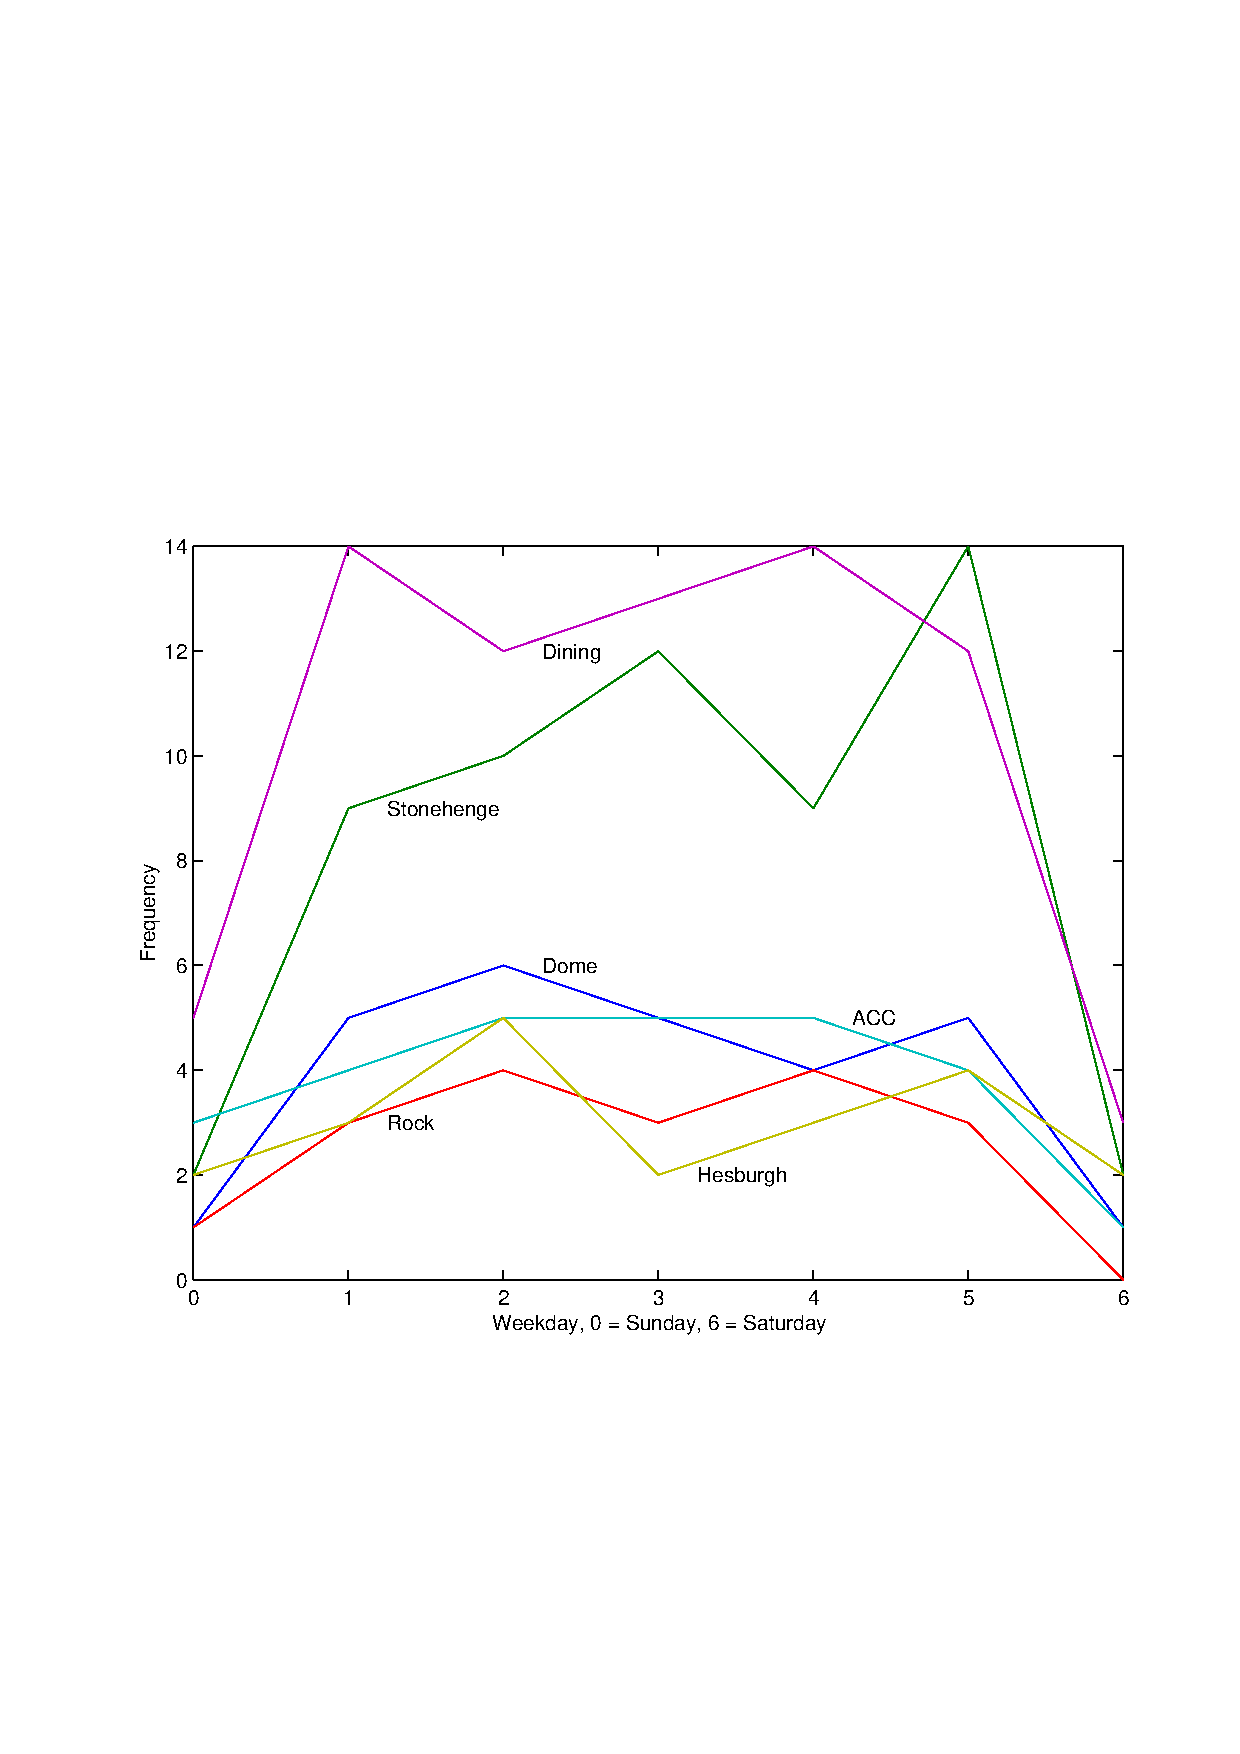
\includegraphics[scale=0.8]{sample_nd}}
    \caption{Location distributions by day of where, where the X axis
      is the weekday (0 through 6), and the Y axis is the sighting
      frequency}
    \label{fig:bogus3}
  \end{center}
\end{figure}

Gnus typically tend to come out when there are large gatherings of
humans with food.  Gnus work very hard at providing us with all the
things that we like (trees, dirt, air, etc.), and so we should freely
give them food.  They will come up and stand a respectful distance
away from you, waiting to see if they will be rewarded for their
efforts.  If you offer some food, they will take it and back off a
respectful distance in order to consume their food while leaving you
to your ``personal space.''  

\section{Groovin' Gnus}
\label{sec:groovin-gnus}

Gnus do tend to stay away from humans in their normal day-to-day
workings.  This is mainly because humans don't, for the most part,
understand what they are doing.  If a Gnu is working, and a human
approaches it, the Gnu will tend to drop whatever it is doing and run
away.  This is probably do to the tendency for humans to have ``group
meetings'' and ``productivity seminars.''  Most Gnus are deathly
afraid of such overmanagement, and run at the slightest hint of it,
for fear that it will cripple their real work.

It is interesting, however, that Gnus have chosen an Institution of
Higher Education for their BOO.\footnote{Base of Operations.}  It is
often said that:
\begin{quote}
  Academic politics are the dirtiest, meanest, ugliest, and generally
  the most low-down, in-your-face, and kick-em-while-they're-down than
  anywhere else (even Washington D.C.)  because the stakes are so low.
\end{quote}
It has been hypothesized that the Gnus are subtly trying to affect a
change for the better (i.e., eliminating the overmanagement problems)
by working the very system that they are trying to change, from
within.  That is, the graduates from Notre Dame can learn from the
examples of the Gnus here, and run screaming (or chattering) at the
slightest hint of overmanagement, and let the real work proceed
unhindered.

% % uncomment the following lines,
% if using chapter-wise bibliography
%
% \bibliographystyle{ndnatbib}
% \bibliography{example}

	\SgIncludeBib{biblio}
\end{document}
\end{lstlisting}

Line 1 simply defines the document class with default options. \\

Lines 4--11 define the variables for automatically creating the title page and setting the PDF document properties. \\

Lines 15--24 defines the front matter of the thesis. \verb|\SgAddTitle| creates the title page using the values of variables defined above. \verb|\SgAddDeclaration| adds the declaration page. Declaration page must be signed. You can either sign after printing or give the path to the signature image as an argument to \verb|\SgAddDeclaration| like this \verb|\SgAddDeclaration[sign-image]|. \verb|%%% Acknowledgements
%%% ----------------------------------------------------------------------
\begingroup
% you can erase the following three lines if you do not use an introductory quote
\cleardoublepage
\let\clearpage\relax
\let\cleardoublepage\relax
\begin{flushright}\slshape
	Put your fancy quote here. Or don't. \\ \medskip
	--- Awesome Author
\end{flushright}

\bigskip
\otherlanguage{ngerman}

\addchap{Vorwort}

\blindmathfalse
\blindtext

\bigskip

\begin{flushright}
	Place, \doctime
\end{flushright}

\endgroup| includes a file containing the acknowledgments. The acknowledgments must be enclosed in \verb|\begin{acknowledgments}| \verb|...| \verb|\end{acknowledgments}|. Similarly, \verb|% !TEX root = main.tex
% !TEX encoding = Windows Latin 1
% !TEX TS-program = pdflatex
% 
% Archivo: abstract.tex (en ingles)


\chapter{Abstract} % No cambiar el titulo
\selectlanguage{english}
\noindent
Duis tristique sollicitudin leo nec consequat. Praesent et dui convallis velit tincidunt fermentum. Mauris cursus purus at sem viverra sed imperdiet sapien imperdiet. Aliquam mattis, elit eget rutrum vulputate, tortor sem pulvinar justo, sit amet mollis felis sem at nibh. Donec malesuada, neque id interdum eleifend, arcu augue porta elit, nec tristique libero metus at massa. Fusce fringilla laoreet rhoncus. Suspendisse potenti. Phasellus dignissim sodales mauris at pharetra. Donec gravida fringilla velit ac rutrum.

Curabitur ornare lectus id diam molestie eu imperdiet nulla tempus. Maecenas vestibulum enim et dui ornare blandit. Vivamus fermentum faucibus viverra. Maecenas at justo sapien. Aenean rhoncus augue mattis purus rhoncus venenatis. Suspendisse metus felis, porttitor in varius in, vulputate at tortor. Aliquam molestie, turpis et malesuada porta, tortor sapien pharetra sapien, ac rhoncus quam dolor a sapien. Pellentesque varius laoreet enim ut auctor. Nullam nec ultricies nisi. Nullam porta lectus et ante consectetur posuere.

Duis tristique sollicitudin leo nec consequat. Praesent et dui convallis velit tincidunt fermentum. Mauris cursus purus at sem viverra sed imperdiet sapien imperdiet. Aliquam mattis, elit eget rutrum vulputate, tortor sem pulvinar justo, sit amet mollis felis sem at nibh. Donec malesuada, neque id interdum eleifend, arcu augue porta elit, nec tristique libero metus at massa. Fusce fringilla laoreet rhoncus. Suspendisse potenti. Phasellus dignissim sodales mauris at pharetra. Donec gravida fringilla velit ac rutrum.

Duis tristique sollicitudin leo nec consequat. Praesent et dui convallis velit tincidunt fermentum. Mauris cursus purus at sem viverra sed imperdiet sapien imperdiet. Aliquam mattis, elit eget rutrum vulputate, tortor sem pulvinar justo, sit amet mollis felis sem at nibh. Donec malesuada, neque id interdum eleifend, arcu augue porta elit, nec tristique libero metus at massa. Fusce fringilla laoreet rhoncus. Suspendisse potenti. Phasellus dignissim sodales mauris at pharetra. Donec gravida fringilla velit ac rutrum.

Curabitur ornare lectus id diam molestie eu imperdiet nulla tempus. Maecenas vestibulum enim et dui ornare blandit. Vivamus fermentum faucibus viverra. Maecenas at justo sapien. Aenean rhoncus augue mattis purus rhoncus venenatis. Suspendisse metus felis, porttitor in varius in, vulputate at tortor. Aliquam molestie, turpis et malesuada porta, tortor sapien pharetra sapien, ac rhoncus quam dolor a sapien. Pellentesque varius laoreet enim ut auctor. Nullam nec ultricies nisi. Nullam porta lectus et ante consectetur posuere.

Duis tristique sollicitudin leo nec consequat. Praesent et dui convallis velit tincidunt fermentum. Mauris cursus purus at sem viverra sed imperdiet sapien imperdiet. Aliquam mattis, elit eget rutrum vulputate, tortor sem pulvinar justo, sit amet mollis felis sem at nibh. Donec malesuada, neque id interdum eleifend, arcu augue porta elit, nec tristique libero metus at massa. Fusce fringilla laoreet rhoncus. Suspendisse potenti. Phasellus dignissim sodales mauris at pharetra. Donec gravida fringilla velit ac rutrum.

\bigskip
\noindent
\textit{Key words:} first word; second word; third word.
% Separar palabras con punto-y-comas.

\checklanguage
% Fin archivo abstract.tex
\endinput | includes a file containing the abstract. The abstract must be enclosed in \verb|\begin{abstract}| \verb|...| \verb|\end{abstract}|. Note that it is not necessary to create separate files for acknowledgments and abstract and they can be inserted inline. \\

Lines 20--23 inserts the table of contents, list of figures, list of tables, and list of algorithms. The order of list of figures, list of tables, and list of algorithms can be changed and not all of the them are necessary. \\

After the front matter is specified, you are free to add main content of the thesis. You can either create one tex file per chapter and include them using \verb|\input{}| or simply include everything in the main file. You can see example\textbackslash{}figure.tex, example\textbackslash{}table.tex, example\textbackslash{}algorithm.tex for examples of how to include figures, tables, and algorithms, respectively. \\

Finally, the bibliography should be included using \verb|\SgIncludeBib{}|. If your bibliography is divided in multiple files, than they can be separated by comma (,).

\section{Class options}\label{sec:ClassOptions}
\SPhdThesis document class uses key=value format for specifying options. Two options are separated by a comma (,). For example \verb|\documentclass[media=print,title=upper]{SPhdThesis}|. The following options are provided:\\

\noindent\textbf{Media type}\\
\Code{media} = \Code{screen} or \Code{print} (default value is \Code{screen}). \Code{media} internally defines the formatting settings for viewing document on screen or printing. When formatting for screen, colors are used for links, tables, and algorithms whereas only black color is used for them in the print mode.\\

\noindent\textbf{Title page casing:}\\
\Code{titlecase} = \Code{lower} or \Code{upper} (default is \Code{upper}). NUS requires the title page to be formatted in uppercase but I don't like uppercase. So, I used this option to format the title page in the lowercase everywhere expect the final submission.\\

\noindent\textbf{Line spacing:}\\
\Code{linespacing} = \Code{onehalf} or \Code{double} (default is \Code{onehalf}). NUS requires the thesis to be formatted with double line spacing which in my opinion doesn’t look very good. So, I used this option to format the thesis with one half line spacing everywhere expect the final submission.\\

\noindent\textbf{Font size:}\\
\Code{fontsize} = \Code{11pt} or \Code{12pt} (default is \Code{11pt}). NUS recommends font size to be 11 or 12 points. This option can be used to format the thesis in either 11 or 12 points. \\

\noindent\textbf{Open type:}\\
\Code{open} = \Code{right} or \Code{any} (default value is \Code{any}). This option defines which page a new chapter will start from: for \Code{open}{}=\Code{any} a new chapter will start from the next new page. However, for \Code{open}{}=\Code{right} a new chapter will only start from next right hand side (odd) page.

\section{Tweaking the document class}\label{sec:Tweaking}
The \verb|SPhdThesis.cls| file is heavily commented and should be mostly easy to understand. It is divided into sections and the order of some sections are important. For example, captions section should come before packages and hyperref section. All these dependencies are documented in the \verb|SPhdThesis.cls| file. \\

Here are some hints to customize the formatting of the thesis:
\begin{itemize}
	\item Chapter and section title formatting: The appearance of chapter and section title in various places in the thesis is defined in the fonts section. The variables defined in the font section are used by TOC (for formatting table of contents), chapter heading (for formatting the chapter heading), and fancy header (for formatting the headers and footers) sections.
	\item Chapter heading: The chapter heading is formatted using Lenny style of the fncychap package. If you like to change to another style supported by fncychap package you can do so in chapter heading section.
	\item Page layout: The paper size and margins are defined in the page layout section. Some other important properties defined is the page layout section are: paragraph indenting, footnote spacing, forcing image to be on the top on blank pages, distance between a float and text, and distance between two floats.
	\item Fancy header: The appearance of header is changed using fancyhdr package in the fancy header section. There are three parts in the header: left, center, and right. In SPhdThesis class, Chapter \#. Chapter\_Name appears on the left part and page number appears on the right part.
	\item TOC. The appearance of the table of contents is changed using tocloft package in the TOC section. Dots separating chapter titles and page numbers are removed and the appearance of the chapter title and page number is defined.
	\item Table: The appearance of tables is defined in the table section. Apart from various distance used for format table you can change the color of horizontal rules.
	\item Algorithm: The appearance of algorithms is defined in the algorithm section.
\end{itemize}

\section{Known Issues}\label{sec:Issues}
\begin{itemize}
	\item Color of rules in algorithms, unlike tables, are black in both print and screen mode.
\end{itemize}

\section{Tools}\label{sec:Tools}
Some tools which are useful for working with \LaTeX:
\begin{itemize}
	\item \textbf{The Ipe extensible drawing editor}\\
	Ipe is a drawing editor for creating figures in PDF or (encapsulated) Postscript format. It supports making small figures for inclusion into LaTeX-documents as well as making multi-page PDF presentations that can be shown on-line with Acrobat Reader.\\
Website: \url{http://ipe7.sourceforge.net/}
	\item \textbf{Jabref reference manager}\\
	JabRef is an open source bibliography reference manager. The native file format used by JabRef is BibTeX, the standard LaTeX bibliography format. JabRef runs on the Java VM (version 1.6 or newer), and should work equally well on Windows, Linux and Mac OS X.\\
	Website: \url{http://jabref.sourceforge.net/}
	\item \textbf{Gle - Graphics Layout Engine}\\
	GLE (Graphics Layout Engine) is a graphics scripting language designed for creating publication quality figures (e.g., a chart, plot, graph, or diagram). It supports various chart types (including function plot, histogram, bar chart, scatter plot, contour plot, color map, and surface plot) through a simple but flexible set of graphing commands. More complex output can be created by relying on GLE's scripting language, which is full featured with subroutines, variables, and logic control. GLE relies on LaTeX for text output and supports mathematical formulae in graphs and figures. GLE's output formats include EPS, PS, PDF, JPEG, and PNG.\\
	Website: \url{http://glx.sourceforge.net/}
	\item \textbf{Chktex - \LaTeX semantic checker}\\
	Chktex is a tool for catching typographic errors in a latex document.\\
	Website: \url{http://baruch.ev-en.org/proj/chktex/}
	\item \textbf{lacheck - \LaTeX checker}\\
	Lacheck is a tool for finding common mistakes in \LaTeX documents.\\
	Website: \url{http://www.ctan.org/tex-archive/support/lacheck}
\end{itemize}

\end{document}
